%\documentclass{article}
%\pagestyle{empty}
%\usepackage{tikz}

\tikzstyle{vertex} = [fill,shape=circle,node distance=80pt]
\tikzstyle{edge} = [fill,opacity=.5,fill opacity=.5,line cap=round, line join=round, line width=50pt]
\tikzstyle{elabel} =  [fill,shape=circle,node distance=35pt]

\pgfdeclarelayer{background}
\pgfsetlayers{background,main}

%\begin{document}
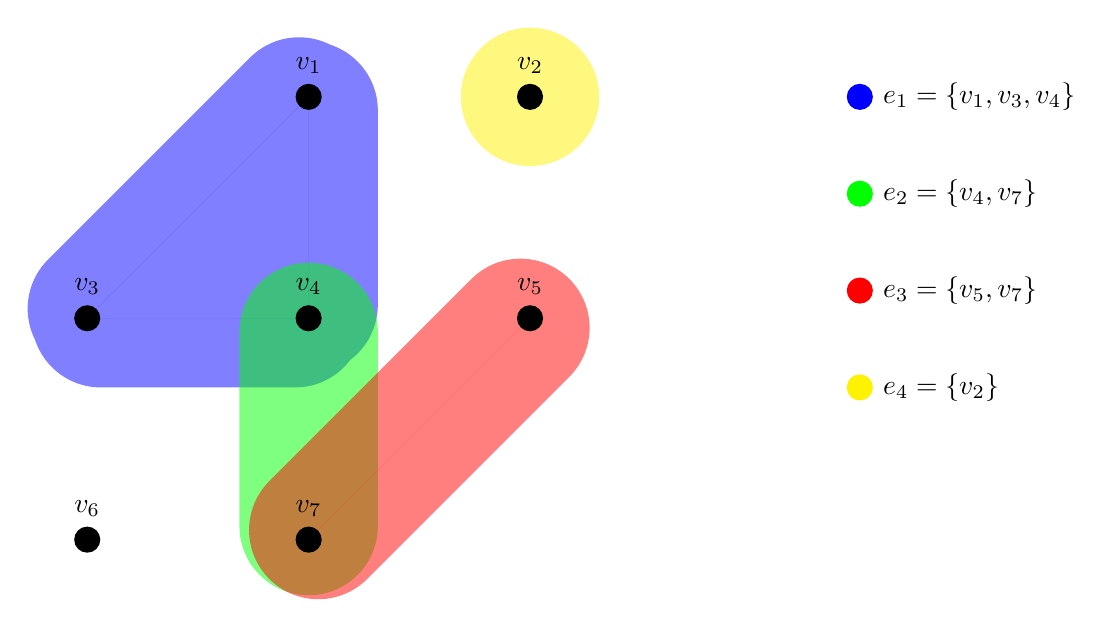
\begin{tikzpicture}
\node[vertex,label=above:\(v_1\)] (v1) {};
\node[vertex,right of=v1,label=above:\(v_2\)] (v2) {};
\node[vertex,below of=v1,label=above:\(v_4\)] (v4) {};
\node[vertex,right of=v4,label=above:\(v_5\)] (v5) {};
\node[vertex,left of=v4,label=above:\(v_3\)] (v3) {};
\node[vertex,below of=v4,label=above:\(v_7\)] (v7) {};
\node[vertex,left of=v7,label=above:\(v_6\)] (v6) {};

\begin{pgfonlayer}{background}
\draw[edge,color=blue] (v1) -- (v3) -- (v4) -- (v1);
\begin{scope}[transparency group,opacity=.5]
\draw[edge,opacity=1,color=green] (v4) -- (v7);
%\fill[edge,opacity=1,color=green] (v3.center) -- (v5.center) -- (v6.center) -- (v3.center);
\end{scope}
\draw[edge,color=red] (v5) -- (v7);
\draw[edge,color=yellow] (v2) -- (v2);
%\draw[edge,color=blue] (v6) -- (v6);
\end{pgfonlayer}

\node[elabel,color=blue,label=right:{$e_1=\{v_1,v_3,v_4\}$}]  (e1) at (7,0) {};
\node[elabel,below of=e1,color=green,label=right:{$e_2=\{v_4,v_7 \}$}]  (e2) {};
\node[elabel,below of=e2,color=red,label=right:{$e_3=\left\{ v_5,v_7 \right\}$}]  (e3) {};
\node[elabel,below of=e3,color=yellow,label=right:{$e_4=\left\{ v_2 \right\}$}]  (e4) {};
\end{tikzpicture}
%\end{document}
